
As Matrizes Curriculares apresentam quais disciplinas o aluno precisa cumprir para a conclusão de determinado curso. Cada unidade curricular possui uma ementa constituída pelos objetivos da disciplina, perfil dos ingressantes (pré-requisitos), e bibliografia básica e complementar. Os alunos das Universidades Federais brasileiras, mais especificamente, os alunos da Universidade de Brasília possuem grande dificuldade em selecionar a grade de disciplinas a serem cursadas no semestre seguinte. Esta dificuldade só é possível graças a flexibilidade da matriz curricular dos cursos da UnB. A UnB exige que 70\% do curso seja composto de disciplinas obrigatórias, formando a estrutura central do curso. Os 30\% restantes podem ser distribuidos em disciplinas optativas a escolha do Aluno. Dessa forma, os próprios alunos desenham o seu curso a partir de seu interesse em determinadas áreas. Assim são formadas as ênfases durante o curso, por exemplo.

O fluxo curricular e as ementas das disciplinas são de fundamental importância no processo de matrícula do aluno. No entanto, no contexto da Universidade de Brasília (UnB), há uma deficiência na apresentação dessas informações, resultando em dificuldades na obtenção de informações referentes às disciplinas e de relações entre as elas. No contexto específico à Faculdade do Gama (FGA), existe grande mutabilidade em relação às matrizes curriculares. A constante alteração no fluxo é um agravante para a pobre representação de informações. 

Tais fatores levam a dificuldades no processo de matrícula. Além da confusão no controle do fluxo curricular, o aluno não possui auxílio ou base de comparação para a escolha de disciplinas optativas, o que pode levar à matrícula em disciplinas que não se encaixam em seu perfil. Falta de interesse e baixo rendimento são só algumas das consequências.

O problema se enquadra na ausência de uma representação semântica das informações Curriculares dos cursos de Engenharia da Universidade de Brasília - UnB Gama e de todas as Universidades brasileiras. Todo o trabalho de oferta e análise se baseia em nomes elencados e fluxos estáticos, não havendo nenhum sentido ou significado envolvidos. A abrangência deste problema vai deste ensino público até privado, englobando, todos os cursos e universidades que não possuem representação semântica de deus Currículos. O foco deste trabalho será no estudo do problema relacionado exclusivamente a Universidade de Brasília - Campus Gama, porém este estudo gera um \textit{input} muito importante para a solução de diversos outros contextos. 

Como o objetivo de apresentar o Problema a ser atacado de forma clara, foi utilizada a técnica do Diagrama de Ishikawa, que pode ser observada na imagem \ref{img:fishbone}.

\begin{figure}[H]
	\centering
	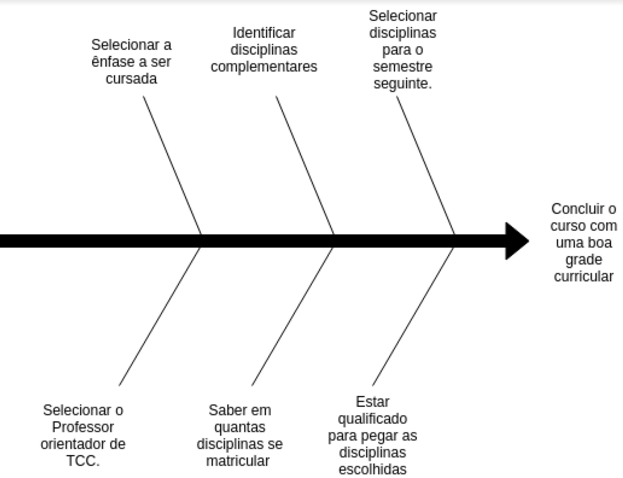
\includegraphics[width=0.8\textwidth]{imagens/fishbone}
	\caption{Diagrama de Fishbone}
	\label{img:fishbone}
\end{figure}
